\documentclass[border=14pt]{standalone}
\usepackage{tikz}
\usetikzlibrary{arrows.meta,decorations.markings,3d}
\usepackage{amsmath}

\begin{document}
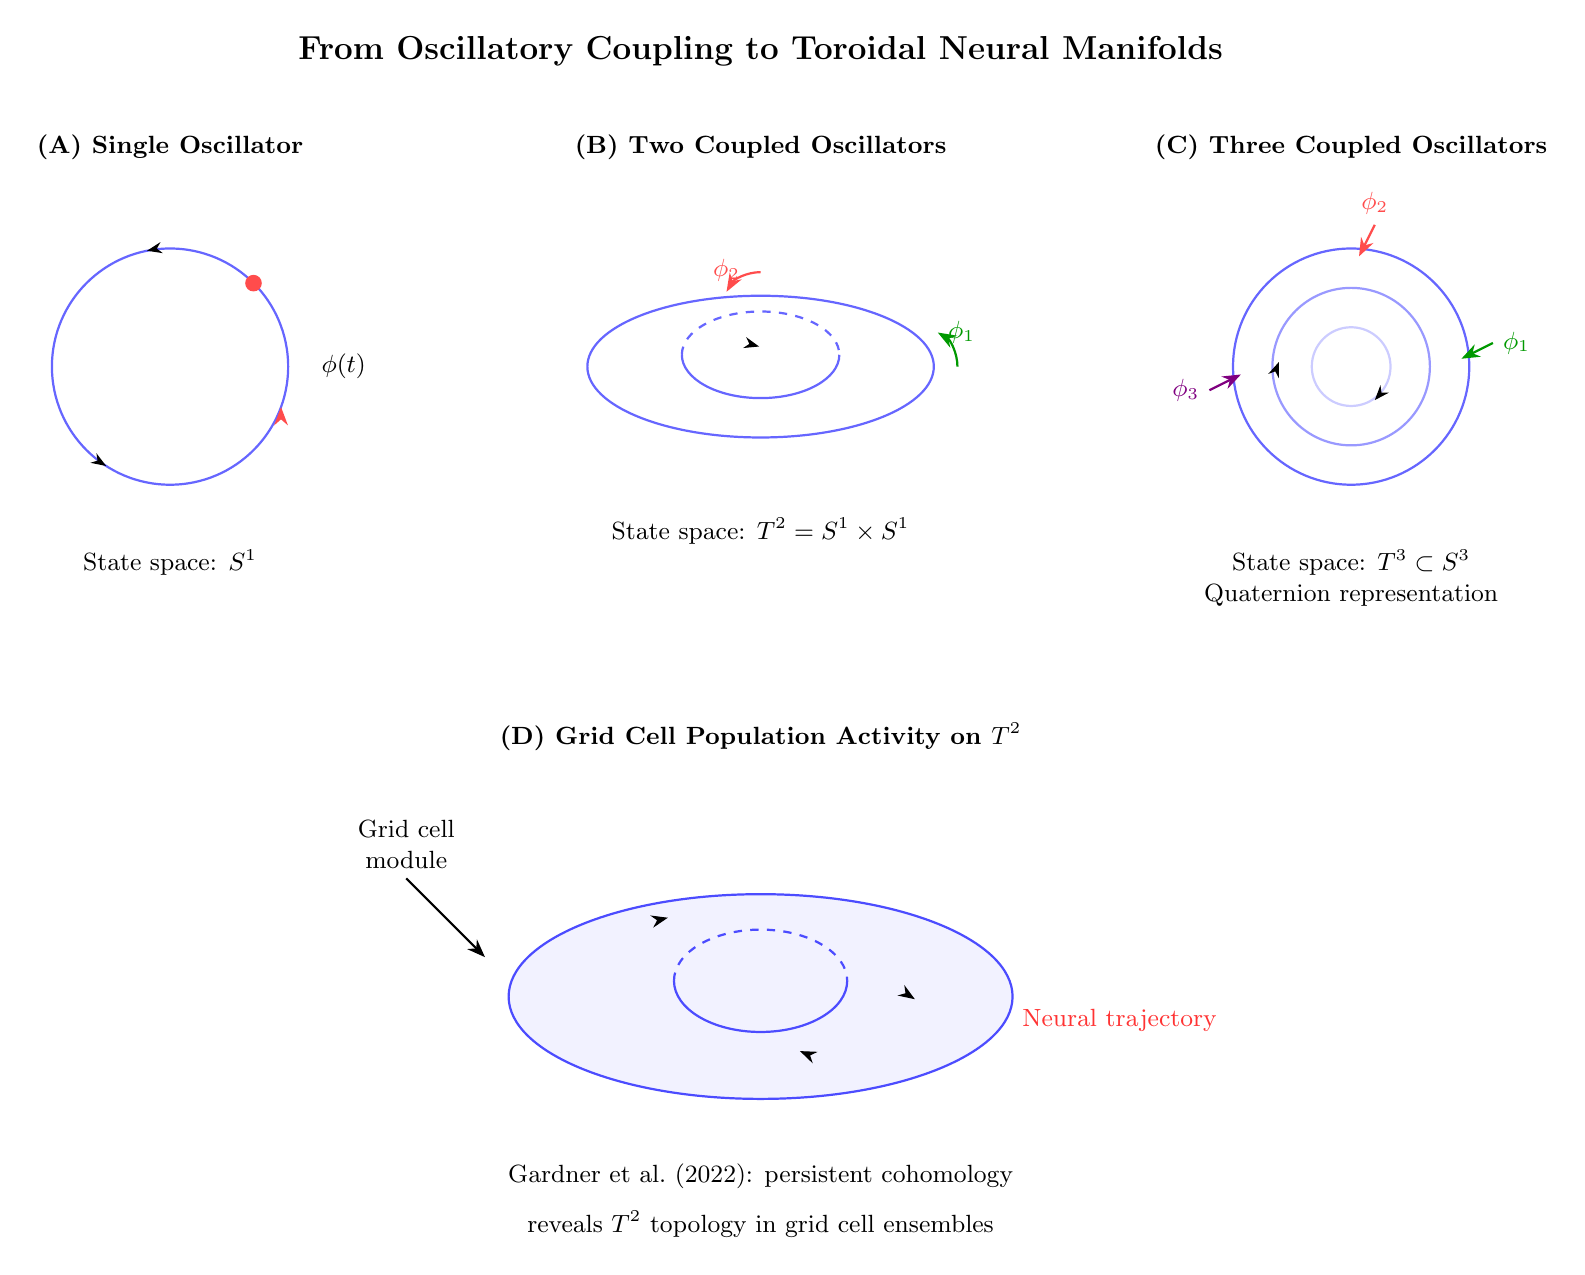
\begin{tikzpicture}[>=Stealth, font=\small]

% Title
\node[font=\large\bfseries] at (0,7.5) {From Oscillatory Coupling to Toroidal Neural Manifolds};

% --- Panel A: Single oscillator -> circle ---
\begin{scope}[shift={(-7.5,3.5)}]
  \node[above, font=\small\bfseries] at (0,2.5) {(A) Single Oscillator};
  \draw[thick, blue!60] (0,0) circle (1.5);
  \draw[->, thick, red!70, decorate, decoration={markings, mark=at position 0.3 with {\arrow{>}}, mark=at position 0.7 with {\arrow{>}}}] 
    (1.5,0) arc (0:340:1.5);
  \node[right] at (1.8,0) {$\phi(t)$};
  \fill[red!70] (1.06,1.06) circle (3pt);
  \node[below, font=\small] at (0,-2.2) {State space: $S^1$};
\end{scope}

% --- Panel B: Two coupled oscillators -> torus ---
\begin{scope}[shift={(0,3.5)}]
  \node[above, font=\small\bfseries] at (0,2.5) {(B) Two Coupled Oscillators};
  % Draw torus outline (simplified)
  \draw[thick, blue!60] (0,0) ellipse (2.2 and 0.9);
  \draw[thick, blue!60] (-1.0,0.15) arc (180:360:1.0 and 0.55);
  \draw[thick, blue!60, dashed] (-1.0,0.15) arc (180:0:1.0 and 0.55);
  % Phase arrows
  \draw[->, thick, green!60!black] (2.5,0) arc (0:60:0.5) node[right, font=\small] {$\phi_1$};
  \draw[->, thick, red!70] (0,1.2) arc (90:150:0.5) node[above, font=\small] {$\phi_2$};
  % Trajectory hint
  \draw[thick, orange, dashed, decorate, decoration={markings, mark=at position 0.5 with {\arrow{>}}}] 
    (-1.7,0.3) .. controls (-0.5,0.8) and (0.5,-0.3) .. (1.7,0.2);
  \node[below, font=\small] at (0,-1.8) {State space: $T^2 = S^1 \times S^1$};
\end{scope}

% --- Panel C: Three coupled -> quaternion S^3 ---
\begin{scope}[shift={(7.5,3.5)}]
  \node[above, font=\small\bfseries] at (0,2.5) {(C) Three Coupled Oscillators};
  % Draw hypersphere projection (simplified as nested circles)
  \draw[thick, blue!60] (0,0) circle (1.5);
  \draw[thick, blue!40] (0,0) circle (1.0);
  \draw[thick, blue!20] (0,0) circle (0.5);
  % Phase arrows
  \draw[->, thick, green!60!black] (1.8,0.3) node[right, font=\small] {$\phi_1$} -- (1.4,0.1);
  \draw[->, thick, red!70] (0.3,1.8) node[above, font=\small] {$\phi_2$} -- (0.1,1.4);
  \draw[->, thick, violet] (-1.8,-0.3) node[left, font=\small] {$\phi_3$} -- (-1.4,-0.1);
  % Trajectory
  \draw[thick, orange, dashed, decorate, decoration={markings, mark=at position 0.3 with {\arrow{>}}, mark=at position 0.7 with {\arrow{>}}}] 
    (0.5,1.4) .. controls (1.2,0.5) and (0.3,-1.0) .. (-1.0,-1.1) .. controls (-1.3,0.2) and (-0.2,1.3) .. (0.5,1.4);
  \node[below, align=center, font=\small] at (0,-2.2) {State space: $T^3 \subset S^3$\\Quaternion representation};
\end{scope}

% --- Panel D: Grid cell toroidal manifold ---
\begin{scope}[shift={(0,-4.5)}]
  \node[above, font=\small\bfseries] at (0,3.0) {(D) Grid Cell Population Activity on $T^2$};
  
  % Draw a torus
  \draw[thick, blue!70, fill=blue!5] (0,0) ellipse (3.2 and 1.3);
  \draw[thick, blue!70] (-1.1,0.2) arc (180:360:1.1 and 0.65);
  \draw[thick, blue!70, dashed] (-1.1,0.2) arc (180:0:1.1 and 0.65);
  
  % Trajectory on torus
  \draw[very thick, red!80, decorate, decoration={markings, 
    mark=at position 0.15 with {\arrow{>}}, 
    mark=at position 0.45 with {\arrow{>}},
    mark=at position 0.75 with {\arrow{>}}}] 
    (-2.7,0.3) .. controls (-1.5,1.1) and (-0.3,1.3) .. (0.5,0.9) 
    .. controls (1.3,0.4) and (2.2,-0.2) .. (2.7,-0.5)
    .. controls (3.0,-0.8) and (2.2,-1.1) .. (1.0,-0.9)
    .. controls (0,-0.5) and (-1.0,0.0) .. (-2.2,0.4);
  
  % Labels
  \node[right, red!80, font=\small] at (3.2,-0.3) {Neural trajectory};
  
  % Module label
  \draw[<-, thick] (-3.5,0.5) -- (-4.5,1.5) node[above, align=center, font=\small] {Grid cell\\module};
  
  % Citation below
  \node[below, align=center, font=\small] at (0,-2.0) {Gardner et al.\ (2022): persistent cohomology};
  \node[below, align=center, font=\small] at (0,-2.6) {reveals $T^2$ topology in grid cell ensembles};
\end{scope}

\end{tikzpicture}
\end{document}
